\documentclass[12pt,a4paper]{article}

\usepackage[utf8]{inputenc}
\usepackage[T1]{fontenc}
\usepackage[english]{babel}
\usepackage{lmodern}
\usepackage[left=2cm,right=1.5cm,top=2cm,bottom=2cm]{geometry}
\usepackage{setspace}
\usepackage{graphicx}
\usepackage{xcolor}
\usepackage{listings}
\usepackage{titlesec}
\usepackage{caption}
\usepackage{float}
\usepackage{booktabs}
\usepackage{array}
\usepackage{fancyhdr}
\usepackage{needspace}
\usepackage[hidelinks]{hyperref}

\graphicspath{{figures/}}
\onehalfspacing
\setlength{\parindent}{1.25cm}
\setlength{\parskip}{0pt}
\setlength{\emergencystretch}{2em}

\definecolor{cipherbackground}{HTML}{F7F7F7}
\definecolor{cipherframe}{HTML}{CBD5E1}
\definecolor{resolvedgreen}{HTML}{166534}
\definecolor{headingblue}{HTML}{1E3A5F}
\definecolor{plaintextbackground}{HTML}{F3F8F4}

\titleformat{\section}
  {\normalfont\bfseries\centering\fontsize{13}{16}\selectfont}
  {\thesection}{0.8em}{\MakeUppercase}
\titleformat{name=\section,numberless}
  {\normalfont\bfseries\centering\fontsize{13}{16}\selectfont}
  {}{0pt}{\MakeUppercase}
\titleformat{\subsection}
  {\normalfont\bfseries\fontsize{12}{15}\selectfont}
  {\thesubsection}{0.7em}{}
\titlespacing*{\section}{0pt}{0pt}{12pt}
\titlespacing*{\subsection}{0pt}{10pt}{6pt}

\pagestyle{fancy}
\fancyhf{}
\fancyhead[L]{\small\textit{Cryptography and Security}}
\fancyhead[R]{\small Laboratory Work No. 2}
\fancyfoot[C]{\thepage}
\renewcommand{\headrulewidth}{0.4pt}
\renewcommand{\footrulewidth}{0pt}
\setlength{\headheight}{15pt}

\lstdefinestyle{ciphertext}{
  basicstyle=\ttfamily\fontsize{8.2}{10.2}\selectfont,
  backgroundcolor=\color{cipherbackground},
  frame=single,
  rulecolor=\color{cipherframe},
  breaklines=true,
  breakatwhitespace=true,
  columns=fullflexible,
  keepspaces=true,
  showstringspaces=false,
  xleftmargin=0.25cm,
  xrightmargin=0.15cm,
  framexleftmargin=0.15cm,
  framesep=5pt,
  aboveskip=7pt,
  belowskip=7pt,
  captionpos=b
}

\lstdefinestyle{plaintext}{
  style=ciphertext,
  basicstyle=\ttfamily\fontsize{8.5}{10.5}\selectfont,
  backgroundcolor=\color{plaintextbackground},
  rulecolor=\color{resolvedgreen}
}

\newcommand{\caselegend}{%
  \noindent\textbf{Reading convention: }
  \texttt{CAPITALS} are unresolved ciphertext symbols; 
  \texttt{lowercase} letters are confirmed plaintext substitutions.\par
}

\begin{document}

\begin{titlepage}
  \thispagestyle{empty}
  \begin{center}
    
\includegraphics[width=3.4cm]{LOGO_UTM.jpg}\par
    \vspace{0.25cm}

    {\bfseries\fontsize{14}{17}\selectfont
      MINISTRY OF EDUCATION AND RESEARCH\par
      OF THE REPUBLIC OF MOLDOVA\par
      Technical University of Moldova\par
      Faculty of Computers, Informatics and Microelectronics\par
      Department of Software Engineering and Automation\par
    }

    \vspace{1.4cm}
    {\bfseries\fontsize{16}{19}\selectfont Daniel Moisei, FAF-241\par}

    \vspace{1.4cm}
    {\bfseries\fontsize{36}{40}\selectfont Report\par}
    \vspace{0.25cm}
    {\itshape\fontsize{20}{24}\selectfont Laboratory Work No. 2\par}
    {\bfseries\itshape\fontsize{20}{24}\selectfont Cryptography and Security\par}

    \vspace{1cm}
    {\fontsize{20}{25}\selectfont Topic: Cryptanalysis of Monoalphabetic Ciphers\par}
    \vspace{0.2cm}
    {\fontsize{15}{19}\selectfont Frequency Analysis of Variant 17\par}
  \end{center}

  \vfill
  \begin{flushright}
    {\fontsize{15}{18}\selectfont Checked by:}\par
    \textbf{Maia Zaica}, \textit{university assistant}
  \end{flushright}

  \vfill
  \begin{center}
    {\bfseries\fontsize{14}{17}\selectfont Chi\c{s}in\u{a}u -- 2026}
  \end{center}
\end{titlepage}

\pagenumbering{arabic}
\setcounter{page}{2}
\tableofcontents
\newpage

\section*{Introduction}
\addcontentsline{toc}{section}{Introduction}

The purpose of this laboratory work is to recover an English plaintext encrypted with a monoalphabetic substitution cipher. I solved Variant 17 manually with the frequency-analysis service specified in the laboratory handout. The attack combines letter frequencies with repeated patterns, common short words, and contextual recognition.

At every stage below, confirmed plaintext letters are shown in lowercase while unresolved ciphertext symbols remain uppercase. This makes the progress of the attack visible and reproduces the notation used by the online tool. The complete text is included after every iteration, as required by the worked-example format in the handout.

\newpage
\section{Short Theory}

\subsection{Monoalphabetic Substitution}

In a monoalphabetic substitution cipher, every plaintext letter is replaced by one fixed ciphertext letter. The key is therefore a permutation of the alphabet. For plaintext letter $x$ and substitution permutation $\pi$, encryption and decryption can be written as

\begin{equation}
  y=\pi(x), \qquad x=\pi^{-1}(y).
\end{equation}

Spaces, punctuation, and digits are not encrypted in this task. Although there are $26!$ possible alphabet permutations, the cipher preserves the statistical structure of the language: a frequent plaintext letter still produces a frequent ciphertext symbol, repeated letters remain repeated, and identical word patterns remain visible.

\subsection{Frequency and Pattern Analysis}

English text has a characteristic distribution in which e, t, a, o, i, and n are among the most common letters. Frequency comparison provides hypotheses, but it is not sufficient by itself because a finite passage differs from the ideal distribution. The hypotheses must be checked against common digraphs such as th and he, common trigraphs such as the and and, one-letter words, word lengths, repeated-letter patterns, and the meaning of the surrounding sentence.

The practical attack is iterative. A plausible substitution is entered, the entire text is updated, and newly visible word fragments provide evidence for the next substitution. Incorrect hypotheses can be reversed; a correct hypothesis normally completes several patterns at once.

\newpage
\section{Frequency Analysis of Variant 17}

\subsection{Initial Intercept}

The intercepted ciphertext supplied for Variant 17 is shown below. The line wrapping is only for readability and does not change the message.
\caselegend
\begin{lstlisting}[style=ciphertext,caption={Variant 17 intercepted ciphertext}]
QTO WQV UIVPXOVGW IVHNZZVGOVO QXP NRG PFPWVZ WN PVHIVWTIF NC PWTWVETZVP ZTOXPNG, QV RNDSO
QTKV VGONRVO QXP HNDGWIF RXWQ T ZVWQNO NCPVHIVW HNZZDGXHTWXNG WQTW RNDSO TSZNPW HVIWTXGSF
QTKV RXWQPWNNO TGFHIFUWTGTSFWXH TWWTHL NC WQNPV OTFP. XGPWVTO QV TUUVTIP WN QTKV CXSVO
TGOCNIJNWWVG XW. XW RTP GNW IVOXPHNKVIVO TZNGJ QXP UTUVIP XG WQV SXAITIF NCHNGJIVPP DGWXS
1922, HNXGHXOVGWTSSF WQV FVTI WQV D.P. TIZF TONUWVO TGTSZNPW XOVGWXHTS OVKXHV WQTW QTO AVVG
XGOVUVGOVGWSF XGKVGWVO. STWVI,NWQVI AITGHQVP NC WQV TZVIXHTG JNKVIGZVGW DPVO WQV
EVCCVIPNG PFPWVZ,JVGVITSSF PSXJQWSF ZNOXCXVO, TGO XW NCWVG OVCVTWVO WQV AVPW VCCNIWP NC
WQV20WQ-HVGWDIF HIFUWTGTSFPWP RQN WIXVO WN AIVTL XW ONRG! WN WQXP OTF WQVGTKF DPVP XW.
WQXP XP T IVZTILTASV SNGJVKXWF. PN XZUNIWTGW XP QXP PFPWVZWQTW XW HNGCVIP DUNG EVCCVIPNG WQV
WXWSV NC CTWQVI NC TZVIXHTGHIFUWNJITUQF.HQTISVP RQVTWPWNGV QTO T IVZTILTASF CVIWXSV ZXGO. QV
HNGPWIDHWVO TGVSVHWIXH WVSVJITUQ AVCNIV ZNIPV OXO, XGKVGWVO WQV HNGHVIWXGT, XZUINKVO WQV
OFGTZN, PWDOXVO DGOVIRTWVI WVSVJITUQF,UINODHVO PNZV NC WQV CXIPW PWVIVNPHNUXH OITRXGJP,
UDASXPQVO QTSC T ONMVGUTUVIP NG THNDPWXHP, OXPHDPPVO UQNGVWXHP TGO QFUNWQVWXHTS
PUVTLXGJZTHQXGVP XG UIXGW, HNGODHWVO GDZVINDP VSVHWIXHTS VYUVIXZVGWP, TGOUNUDSTIXMVO T
ZVWQNO CNI WQV VYWIVZVSF THHDITWV ZVTPDIVZVGW NCVSVHWIXHTS IVPXPWTGHV GNR XG CIVBDVGW DPV
TGO HTSSVO WQV "RQVTWPWNGVAIXOJV." QXP RNIL RTP QXJQSF VGNDJQ IVJTIOVO CNI QXZ WN AV VSVHWVO
TCVSSNR NC WQV INFTS PNHXVWF TGO WN AV LGXJQWVO. QV RTP GNZXGTSSFUINCVPPNI NC VYUVIXZVGWTS
UQXSNPNUQF TW LXGJ'P HNSSVJV, SNGONG, ADW RTP PN VYHVPPXKVSF PQF WQTWQV QTIOSF VKVI THWDTSSF
SVHWDIVO.TGNWQVI NC QXP XGKVGWXNGP RTP T HXUQVI CNI PVHIVHF XG WVSVJITUQF,RQXHQ, QNRVKVI,
HTIIXVP WQV GTZV NC QXP CIXVGO SFNG USTFCTXI, CXIPW ATINGUSTFCTXI NC PW. TGOIVRP. T PHXVGWXPW
TGO UDASXH CXJDIV NC KXHWNIXTGVGJSTGO, USTFCTXI RTP TW NGV WXZV NI TGNWQVI OVUDWF PUVTLVI NC
WQVQNDPV NC HNZZNGP, UNPWZTPWVI JVGVITS, TGO UIVPXOVGW NC WQV AIXWXPQTPPNHXTWXNG CNI WQV
TOKTGHVZVGW NC PHXVGHV.USTFCTXI OVZNGPWITWVO RQTW QV HTSSVO "RQVTWPWNGV'P GVRSF-
OXPHNKVIVOPFZZVWIXHTS HXUQVI" TW T OXGGVI XG ETGDTIF, 1854, JXKVG AF WQV UIVPXOVGWNC WQV
JNKVIGXGJ HNDGHXS, SNIO JITGKXSSV. NGV NC WQV JDVPWP RTP BDVVGKXHWNIXT'P QDPATGO, UIXGHV
TSAVIW; TGNWQVI RTP WQV QNZV PVHIVWTIF TGOCDWDIV UIXZV ZXGXPWVI, SNIO UTSZVIPWNG. USTFCTXI
VYUSTXGVO WQV PFPWVZ WNQXZ, TGO, RQXSV XG ODASXG T CVR OTFP STWVI, IVHVXKVO WRN PQNIW SVWWVIP
XGWQV HXUQVI CINZ UTSZVIPWNG TGO JITGKXSSV, PQNRXGJ WQTW ANWQ QTO IVTOXSFZTPWVIVO XW.
\end{lstlisting}

\subsection{Observed Frequencies}

I selected \textit{Find Frequencies} on the specified website. The image compares the standard English distribution with the frequencies of this intercept. The most frequent ciphertext letters are V with 272 occurrences (13.1\%), W with 186 (9.0\%), T with 168 (8.1\%), and G, I, and N with approximately 6.8\% each.

\begin{figure}[H]
  \centering
  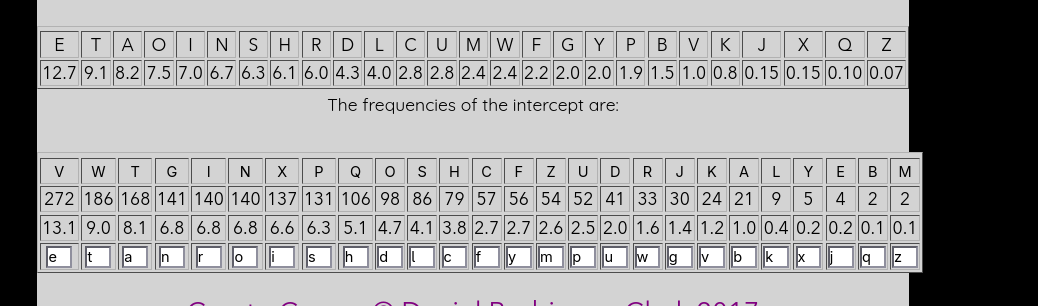
\includegraphics[width=\textwidth]{frequency-analysis.png}
  \caption{Reference English frequencies, Variant 17 frequencies, and the completed substitutions}
  \label{fig:frequency-analysis}
\end{figure}

The high counts provide starting hypotheses, while the words created after each replacement decide whether those hypotheses are credible.

\newpage
\section{Iterative Decoding Process}

Each state below is cumulative. A letter changes to lowercase only in the iteration where its substitution is accepted; every still-undiscovered symbol remains uppercase.

\caselegend
\needspace{7\baselineskip}
\subsection{Iteration 1}

\noindent\textbf{New substitutions:} \texttt{V}$\rightarrow$\texttt{e}.\par
\smallskip
\noindent\textbf{Reasoning.} The frequency tool showed that V is the most common ciphertext letter: 272 occurrences, or 13.1\% of the intercept. Since e is the most frequent English letter, I first tested V as e.

\begin{lstlisting}[style=ciphertext,caption={Complete text after iteration 1}]
QTO WQe UIePXOeGW IeHNZZeGOeO QXP NRG PFPWeZ WN PeHIeWTIF NC PWTWeETZeP ZTOXPNG, Qe RNDSO
QTKe eGONReO QXP HNDGWIF RXWQ T ZeWQNO NCPeHIeW HNZZDGXHTWXNG WQTW RNDSO TSZNPW HeIWTXGSF
QTKe RXWQPWNNO TGFHIFUWTGTSFWXH TWWTHL NC WQNPe OTFP. XGPWeTO Qe TUUeTIP WN QTKe CXSeO
TGOCNIJNWWeG XW. XW RTP GNW IeOXPHNKeIeO TZNGJ QXP UTUeIP XG WQe SXAITIF NCHNGJIePP DGWXS
1922, HNXGHXOeGWTSSF WQe FeTI WQe D.P. TIZF TONUWeO TGTSZNPW XOeGWXHTS OeKXHe WQTW QTO AeeG
XGOeUeGOeGWSF XGKeGWeO. STWeI,NWQeI AITGHQeP NC WQe TZeIXHTG JNKeIGZeGW DPeO WQe
EeCCeIPNG PFPWeZ,JeGeITSSF PSXJQWSF ZNOXCXeO, TGO XW NCWeG OeCeTWeO WQe AePW eCCNIWP NC
WQe20WQ-HeGWDIF HIFUWTGTSFPWP RQN WIXeO WN AIeTL XW ONRG! WN WQXP OTF WQeGTKF DPeP XW.
WQXP XP T IeZTILTASe SNGJeKXWF. PN XZUNIWTGW XP QXP PFPWeZWQTW XW HNGCeIP DUNG EeCCeIPNG WQe
WXWSe NC CTWQeI NC TZeIXHTGHIFUWNJITUQF.HQTISeP RQeTWPWNGe QTO T IeZTILTASF CeIWXSe ZXGO. Qe
HNGPWIDHWeO TGeSeHWIXH WeSeJITUQ AeCNIe ZNIPe OXO, XGKeGWeO WQe HNGHeIWXGT, XZUINKeO WQe
OFGTZN, PWDOXeO DGOeIRTWeI WeSeJITUQF,UINODHeO PNZe NC WQe CXIPW PWeIeNPHNUXH OITRXGJP,
UDASXPQeO QTSC T ONMeGUTUeIP NG THNDPWXHP, OXPHDPPeO UQNGeWXHP TGO QFUNWQeWXHTS
PUeTLXGJZTHQXGeP XG UIXGW, HNGODHWeO GDZeINDP eSeHWIXHTS eYUeIXZeGWP, TGOUNUDSTIXMeO T
ZeWQNO CNI WQe eYWIeZeSF THHDITWe ZeTPDIeZeGW NCeSeHWIXHTS IePXPWTGHe GNR XG CIeBDeGW DPe
TGO HTSSeO WQe "RQeTWPWNGeAIXOJe." QXP RNIL RTP QXJQSF eGNDJQ IeJTIOeO CNI QXZ WN Ae eSeHWeO
TCeSSNR NC WQe INFTS PNHXeWF TGO WN Ae LGXJQWeO. Qe RTP GNZXGTSSFUINCePPNI NC eYUeIXZeGWTS
UQXSNPNUQF TW LXGJ'P HNSSeJe, SNGONG, ADW RTP PN eYHePPXKeSF PQF WQTWQe QTIOSF eKeI THWDTSSF
SeHWDIeO.TGNWQeI NC QXP XGKeGWXNGP RTP T HXUQeI CNI PeHIeHF XG WeSeJITUQF,RQXHQ, QNReKeI,
HTIIXeP WQe GTZe NC QXP CIXeGO SFNG USTFCTXI, CXIPW ATINGUSTFCTXI NC PW. TGOIeRP. T PHXeGWXPW
TGO UDASXH CXJDIe NC KXHWNIXTGeGJSTGO, USTFCTXI RTP TW NGe WXZe NI TGNWQeI OeUDWF PUeTLeI NC
WQeQNDPe NC HNZZNGP, UNPWZTPWeI JeGeITS, TGO UIePXOeGW NC WQe AIXWXPQTPPNHXTWXNG CNI WQe
TOKTGHeZeGW NC PHXeGHe.USTFCTXI OeZNGPWITWeO RQTW Qe HTSSeO "RQeTWPWNGe'P GeRSF-
OXPHNKeIeOPFZZeWIXHTS HXUQeI" TW T OXGGeI XG ETGDTIF, 1854, JXKeG AF WQe UIePXOeGWNC WQe
JNKeIGXGJ HNDGHXS, SNIO JITGKXSSe. NGe NC WQe JDePWP RTP BDeeGKXHWNIXT'P QDPATGO, UIXGHe
TSAeIW; TGNWQeI RTP WQe QNZe PeHIeWTIF TGOCDWDIe UIXZe ZXGXPWeI, SNIO UTSZeIPWNG. USTFCTXI
eYUSTXGeO WQe PFPWeZ WNQXZ, TGO, RQXSe XG ODASXG T CeR OTFP STWeI, IeHeXKeO WRN PQNIW SeWWeIP
XGWQe HXUQeI CINZ UTSZeIPWNG TGO JITGKXSSe, PQNRXGJ WQTW ANWQ QTO IeTOXSFZTPWeIeO XW.
\end{lstlisting}
\needspace{7\baselineskip}
\subsection{Iteration 2}

\noindent\textbf{New substitutions:} \texttt{W}$\rightarrow$\texttt{t}, \texttt{Q}$\rightarrow$\texttt{h}.\par
\smallskip
\noindent\textbf{Reasoning.} After the first replacement, the frequent three-letter pattern WQe appeared. It fits the common English word the. This also agrees with W being the second most frequent ciphertext letter, just as t follows e in the reference distribution. Therefore W becomes t and Q becomes h.

\begin{lstlisting}[style=ciphertext,caption={Complete text after iteration 2}]
hTO the UIePXOeGt IeHNZZeGOeO hXP NRG PFPteZ tN PeHIetTIF NC PtTteETZeP ZTOXPNG, he RNDSO
hTKe eGONReO hXP HNDGtIF RXth T ZethNO NCPeHIet HNZZDGXHTtXNG thTt RNDSO TSZNPt HeItTXGSF
hTKe RXthPtNNO TGFHIFUtTGTSFtXH TttTHL NC thNPe OTFP. XGPteTO he TUUeTIP tN hTKe CXSeO
TGOCNIJNtteG Xt. Xt RTP GNt IeOXPHNKeIeO TZNGJ hXP UTUeIP XG the SXAITIF NCHNGJIePP DGtXS
1922, HNXGHXOeGtTSSF the FeTI the D.P. TIZF TONUteO TGTSZNPt XOeGtXHTS OeKXHe thTt hTO AeeG
XGOeUeGOeGtSF XGKeGteO. STteI,NtheI AITGHheP NC the TZeIXHTG JNKeIGZeGt DPeO the
EeCCeIPNG PFPteZ,JeGeITSSF PSXJhtSF ZNOXCXeO, TGO Xt NCteG OeCeTteO the AePt eCCNItP NC
the20th-HeGtDIF HIFUtTGTSFPtP RhN tIXeO tN AIeTL Xt ONRG! tN thXP OTF theGTKF DPeP Xt.
thXP XP T IeZTILTASe SNGJeKXtF. PN XZUNItTGt XP hXP PFPteZthTt Xt HNGCeIP DUNG EeCCeIPNG the
tXtSe NC CTtheI NC TZeIXHTGHIFUtNJITUhF.HhTISeP RheTtPtNGe hTO T IeZTILTASF CeItXSe ZXGO. he
HNGPtIDHteO TGeSeHtIXH teSeJITUh AeCNIe ZNIPe OXO, XGKeGteO the HNGHeItXGT, XZUINKeO the
OFGTZN, PtDOXeO DGOeIRTteI teSeJITUhF,UINODHeO PNZe NC the CXIPt PteIeNPHNUXH OITRXGJP,
UDASXPheO hTSC T ONMeGUTUeIP NG THNDPtXHP, OXPHDPPeO UhNGetXHP TGO hFUNthetXHTS
PUeTLXGJZTHhXGeP XG UIXGt, HNGODHteO GDZeINDP eSeHtIXHTS eYUeIXZeGtP, TGOUNUDSTIXMeO T
ZethNO CNI the eYtIeZeSF THHDITte ZeTPDIeZeGt NCeSeHtIXHTS IePXPtTGHe GNR XG CIeBDeGt DPe
TGO HTSSeO the "RheTtPtNGeAIXOJe." hXP RNIL RTP hXJhSF eGNDJh IeJTIOeO CNI hXZ tN Ae eSeHteO
TCeSSNR NC the INFTS PNHXetF TGO tN Ae LGXJhteO. he RTP GNZXGTSSFUINCePPNI NC eYUeIXZeGtTS
UhXSNPNUhF Tt LXGJ'P HNSSeJe, SNGONG, ADt RTP PN eYHePPXKeSF PhF thTthe hTIOSF eKeI THtDTSSF
SeHtDIeO.TGNtheI NC hXP XGKeGtXNGP RTP T HXUheI CNI PeHIeHF XG teSeJITUhF,RhXHh, hNReKeI,
HTIIXeP the GTZe NC hXP CIXeGO SFNG USTFCTXI, CXIPt ATINGUSTFCTXI NC Pt. TGOIeRP. T PHXeGtXPt
TGO UDASXH CXJDIe NC KXHtNIXTGeGJSTGO, USTFCTXI RTP Tt NGe tXZe NI TGNtheI OeUDtF PUeTLeI NC
thehNDPe NC HNZZNGP, UNPtZTPteI JeGeITS, TGO UIePXOeGt NC the AIXtXPhTPPNHXTtXNG CNI the
TOKTGHeZeGt NC PHXeGHe.USTFCTXI OeZNGPtITteO RhTt he HTSSeO "RheTtPtNGe'P GeRSF-
OXPHNKeIeOPFZZetIXHTS HXUheI" Tt T OXGGeI XG ETGDTIF, 1854, JXKeG AF the UIePXOeGtNC the
JNKeIGXGJ HNDGHXS, SNIO JITGKXSSe. NGe NC the JDePtP RTP BDeeGKXHtNIXT'P hDPATGO, UIXGHe
TSAeIt; TGNtheI RTP the hNZe PeHIetTIF TGOCDtDIe UIXZe ZXGXPteI, SNIO UTSZeIPtNG. USTFCTXI
eYUSTXGeO the PFPteZ tNhXZ, TGO, RhXSe XG ODASXG T CeR OTFP STteI, IeHeXKeO tRN PhNIt SetteIP
XGthe HXUheI CINZ UTSZeIPtNG TGO JITGKXSSe, PhNRXGJ thTt ANth hTO IeTOXSFZTPteIeO Xt.
\end{lstlisting}
\needspace{7\baselineskip}
\subsection{Iteration 3}

\noindent\textbf{New substitutions:} \texttt{N}$\rightarrow$\texttt{o}, \texttt{P}$\rightarrow$\texttt{s}.\par
\smallskip
\noindent\textbf{Reasoning.} The short word tN and the pattern thNPe are naturally read as to and those. These two words determine N as o and P as s.

\begin{lstlisting}[style=ciphertext,caption={Complete text after iteration 3}]
hTO the UIesXOeGt IeHoZZeGOeO hXs oRG sFsteZ to seHIetTIF oC stTteETZes ZTOXsoG, he RoDSO
hTKe eGOoReO hXs HoDGtIF RXth T ZethoO oCseHIet HoZZDGXHTtXoG thTt RoDSO TSZost HeItTXGSF
hTKe RXthstooO TGFHIFUtTGTSFtXH TttTHL oC those OTFs. XGsteTO he TUUeTIs to hTKe CXSeO
TGOCoIJotteG Xt. Xt RTs Got IeOXsHoKeIeO TZoGJ hXs UTUeIs XG the SXAITIF oCHoGJIess DGtXS
1922, HoXGHXOeGtTSSF the FeTI the D.s. TIZF TOoUteO TGTSZost XOeGtXHTS OeKXHe thTt hTO AeeG
XGOeUeGOeGtSF XGKeGteO. STteI,otheI AITGHhes oC the TZeIXHTG JoKeIGZeGt DseO the
EeCCeIsoG sFsteZ,JeGeITSSF sSXJhtSF ZoOXCXeO, TGO Xt oCteG OeCeTteO the Aest eCCoIts oC
the20th-HeGtDIF HIFUtTGTSFsts Rho tIXeO to AIeTL Xt OoRG! to thXs OTF theGTKF Dses Xt.
thXs Xs T IeZTILTASe SoGJeKXtF. so XZUoItTGt Xs hXs sFsteZthTt Xt HoGCeIs DUoG EeCCeIsoG the
tXtSe oC CTtheI oC TZeIXHTGHIFUtoJITUhF.HhTISes RheTtstoGe hTO T IeZTILTASF CeItXSe ZXGO. he
HoGstIDHteO TGeSeHtIXH teSeJITUh AeCoIe ZoIse OXO, XGKeGteO the HoGHeItXGT, XZUIoKeO the
OFGTZo, stDOXeO DGOeIRTteI teSeJITUhF,UIoODHeO soZe oC the CXIst steIeosHoUXH OITRXGJs,
UDASXsheO hTSC T OoMeGUTUeIs oG THoDstXHs, OXsHDsseO UhoGetXHs TGO hFUothetXHTS
sUeTLXGJZTHhXGes XG UIXGt, HoGODHteO GDZeIoDs eSeHtIXHTS eYUeIXZeGts, TGOUoUDSTIXMeO T
ZethoO CoI the eYtIeZeSF THHDITte ZeTsDIeZeGt oCeSeHtIXHTS IesXstTGHe GoR XG CIeBDeGt Dse
TGO HTSSeO the "RheTtstoGeAIXOJe." hXs RoIL RTs hXJhSF eGoDJh IeJTIOeO CoI hXZ to Ae eSeHteO
TCeSSoR oC the IoFTS soHXetF TGO to Ae LGXJhteO. he RTs GoZXGTSSFUIoCessoI oC eYUeIXZeGtTS
UhXSosoUhF Tt LXGJ's HoSSeJe, SoGOoG, ADt RTs so eYHessXKeSF shF thTthe hTIOSF eKeI THtDTSSF
SeHtDIeO.TGotheI oC hXs XGKeGtXoGs RTs T HXUheI CoI seHIeHF XG teSeJITUhF,RhXHh, hoReKeI,
HTIIXes the GTZe oC hXs CIXeGO SFoG USTFCTXI, CXIst ATIoGUSTFCTXI oC st. TGOIeRs. T sHXeGtXst
TGO UDASXH CXJDIe oC KXHtoIXTGeGJSTGO, USTFCTXI RTs Tt oGe tXZe oI TGotheI OeUDtF sUeTLeI oC
thehoDse oC HoZZoGs, UostZTsteI JeGeITS, TGO UIesXOeGt oC the AIXtXshTssoHXTtXoG CoI the
TOKTGHeZeGt oC sHXeGHe.USTFCTXI OeZoGstITteO RhTt he HTSSeO "RheTtstoGe's GeRSF-
OXsHoKeIeOsFZZetIXHTS HXUheI" Tt T OXGGeI XG ETGDTIF, 1854, JXKeG AF the UIesXOeGtoC the
JoKeIGXGJ HoDGHXS, SoIO JITGKXSSe. oGe oC the JDests RTs BDeeGKXHtoIXT's hDsATGO, UIXGHe
TSAeIt; TGotheI RTs the hoZe seHIetTIF TGOCDtDIe UIXZe ZXGXsteI, SoIO UTSZeIstoG. USTFCTXI
eYUSTXGeO the sFsteZ tohXZ, TGO, RhXSe XG ODASXG T CeR OTFs STteI, IeHeXKeO tRo shoIt SetteIs
XGthe HXUheI CIoZ UTSZeIstoG TGO JITGKXSSe, shoRXGJ thTt Aoth hTO IeTOXSFZTsteIeO Xt.
\end{lstlisting}
\needspace{7\baselineskip}
\subsection{Iteration 4}

\noindent\textbf{New substitutions:} \texttt{T}$\rightarrow$\texttt{a}.\par
\smallskip
\noindent\textbf{Reasoning.} The pattern thTt can only reasonably be that in this context. Consequently, T becomes a; its high frequency is also compatible with the English frequency table.

\begin{lstlisting}[style=ciphertext,caption={Complete text after iteration 4}]
haO the UIesXOeGt IeHoZZeGOeO hXs oRG sFsteZ to seHIetaIF oC stateEaZes ZaOXsoG, he RoDSO
haKe eGOoReO hXs HoDGtIF RXth a ZethoO oCseHIet HoZZDGXHatXoG that RoDSO aSZost HeItaXGSF
haKe RXthstooO aGFHIFUtaGaSFtXH attaHL oC those OaFs. XGsteaO he aUUeaIs to haKe CXSeO
aGOCoIJotteG Xt. Xt Ras Got IeOXsHoKeIeO aZoGJ hXs UaUeIs XG the SXAIaIF oCHoGJIess DGtXS
1922, HoXGHXOeGtaSSF the FeaI the D.s. aIZF aOoUteO aGaSZost XOeGtXHaS OeKXHe that haO AeeG
XGOeUeGOeGtSF XGKeGteO. SateI,otheI AIaGHhes oC the aZeIXHaG JoKeIGZeGt DseO the
EeCCeIsoG sFsteZ,JeGeIaSSF sSXJhtSF ZoOXCXeO, aGO Xt oCteG OeCeateO the Aest eCCoIts oC
the20th-HeGtDIF HIFUtaGaSFsts Rho tIXeO to AIeaL Xt OoRG! to thXs OaF theGaKF Dses Xt.
thXs Xs a IeZaILaASe SoGJeKXtF. so XZUoItaGt Xs hXs sFsteZthat Xt HoGCeIs DUoG EeCCeIsoG the
tXtSe oC CatheI oC aZeIXHaGHIFUtoJIaUhF.HhaISes RheatstoGe haO a IeZaILaASF CeItXSe ZXGO. he
HoGstIDHteO aGeSeHtIXH teSeJIaUh AeCoIe ZoIse OXO, XGKeGteO the HoGHeItXGa, XZUIoKeO the
OFGaZo, stDOXeO DGOeIRateI teSeJIaUhF,UIoODHeO soZe oC the CXIst steIeosHoUXH OIaRXGJs,
UDASXsheO haSC a OoMeGUaUeIs oG aHoDstXHs, OXsHDsseO UhoGetXHs aGO hFUothetXHaS
sUeaLXGJZaHhXGes XG UIXGt, HoGODHteO GDZeIoDs eSeHtIXHaS eYUeIXZeGts, aGOUoUDSaIXMeO a
ZethoO CoI the eYtIeZeSF aHHDIate ZeasDIeZeGt oCeSeHtIXHaS IesXstaGHe GoR XG CIeBDeGt Dse
aGO HaSSeO the "RheatstoGeAIXOJe." hXs RoIL Ras hXJhSF eGoDJh IeJaIOeO CoI hXZ to Ae eSeHteO
aCeSSoR oC the IoFaS soHXetF aGO to Ae LGXJhteO. he Ras GoZXGaSSFUIoCessoI oC eYUeIXZeGtaS
UhXSosoUhF at LXGJ's HoSSeJe, SoGOoG, ADt Ras so eYHessXKeSF shF thathe haIOSF eKeI aHtDaSSF
SeHtDIeO.aGotheI oC hXs XGKeGtXoGs Ras a HXUheI CoI seHIeHF XG teSeJIaUhF,RhXHh, hoReKeI,
HaIIXes the GaZe oC hXs CIXeGO SFoG USaFCaXI, CXIst AaIoGUSaFCaXI oC st. aGOIeRs. a sHXeGtXst
aGO UDASXH CXJDIe oC KXHtoIXaGeGJSaGO, USaFCaXI Ras at oGe tXZe oI aGotheI OeUDtF sUeaLeI oC
thehoDse oC HoZZoGs, UostZasteI JeGeIaS, aGO UIesXOeGt oC the AIXtXshassoHXatXoG CoI the
aOKaGHeZeGt oC sHXeGHe.USaFCaXI OeZoGstIateO Rhat he HaSSeO "RheatstoGe's GeRSF-
OXsHoKeIeOsFZZetIXHaS HXUheI" at a OXGGeI XG EaGDaIF, 1854, JXKeG AF the UIesXOeGtoC the
JoKeIGXGJ HoDGHXS, SoIO JIaGKXSSe. oGe oC the JDests Ras BDeeGKXHtoIXa's hDsAaGO, UIXGHe
aSAeIt; aGotheI Ras the hoZe seHIetaIF aGOCDtDIe UIXZe ZXGXsteI, SoIO UaSZeIstoG. USaFCaXI
eYUSaXGeO the sFsteZ tohXZ, aGO, RhXSe XG ODASXG a CeR OaFs SateI, IeHeXKeO tRo shoIt SetteIs
XGthe HXUheI CIoZ UaSZeIstoG aGO JIaGKXSSe, shoRXGJ that Aoth haO IeaOXSFZasteIeO Xt.
\end{lstlisting}
\needspace{7\baselineskip}
\subsection{Iteration 5}

\noindent\textbf{New substitutions:} \texttt{X}$\rightarrow$\texttt{i}, \texttt{G}$\rightarrow$\texttt{n}, \texttt{O}$\rightarrow$\texttt{d}.\par
\smallskip
\noindent\textbf{Reasoning.} The word XGsteaO now fits instead exactly. This supplies three substitutions at once: X becomes i, G becomes n, and O becomes d.

\begin{lstlisting}[style=ciphertext,caption={Complete text after iteration 5}]
had the UIesident IeHoZZended his oRn sFsteZ to seHIetaIF oC stateEaZes Zadison, he RoDSd
haKe endoRed his HoDntIF Rith a Zethod oCseHIet HoZZDniHation that RoDSd aSZost HeItainSF
haKe Rithstood anFHIFUtanaSFtiH attaHL oC those daFs. instead he aUUeaIs to haKe CiSed
andCoIJotten it. it Ras not IedisHoKeIed aZonJ his UaUeIs in the SiAIaIF oCHonJIess DntiS
1922, HoinHidentaSSF the FeaI the D.s. aIZF adoUted anaSZost identiHaS deKiHe that had Aeen
indeUendentSF inKented. SateI,otheI AIanHhes oC the aZeIiHan JoKeInZent Dsed the
EeCCeIson sFsteZ,JeneIaSSF sSiJhtSF ZodiCied, and it oCten deCeated the Aest eCCoIts oC
the20th-HentDIF HIFUtanaSFsts Rho tIied to AIeaL it doRn! to this daF thenaKF Dses it.
this is a IeZaILaASe SonJeKitF. so iZUoItant is his sFsteZthat it HonCeIs DUon EeCCeIson the
titSe oC CatheI oC aZeIiHanHIFUtoJIaUhF.HhaISes Rheatstone had a IeZaILaASF CeItiSe Zind. he
HonstIDHted aneSeHtIiH teSeJIaUh AeCoIe ZoIse did, inKented the HonHeItina, iZUIoKed the
dFnaZo, stDdied DndeIRateI teSeJIaUhF,UIodDHed soZe oC the CiIst steIeosHoUiH dIaRinJs,
UDASished haSC a doMenUaUeIs on aHoDstiHs, disHDssed UhonetiHs and hFUothetiHaS
sUeaLinJZaHhines in UIint, HondDHted nDZeIoDs eSeHtIiHaS eYUeIiZents, andUoUDSaIiMed a
Zethod CoI the eYtIeZeSF aHHDIate ZeasDIeZent oCeSeHtIiHaS IesistanHe noR in CIeBDent Dse
and HaSSed the "RheatstoneAIidJe." his RoIL Ras hiJhSF enoDJh IeJaIded CoI hiZ to Ae eSeHted
aCeSSoR oC the IoFaS soHietF and to Ae LniJhted. he Ras noZinaSSFUIoCessoI oC eYUeIiZentaS
UhiSosoUhF at LinJ's HoSSeJe, Sondon, ADt Ras so eYHessiKeSF shF thathe haIdSF eKeI aHtDaSSF
SeHtDIed.anotheI oC his inKentions Ras a HiUheI CoI seHIeHF in teSeJIaUhF,RhiHh, hoReKeI,
HaIIies the naZe oC his CIiend SFon USaFCaiI, CiIst AaIonUSaFCaiI oC st. andIeRs. a sHientist
and UDASiH CiJDIe oC KiHtoIianenJSand, USaFCaiI Ras at one tiZe oI anotheI deUDtF sUeaLeI oC
thehoDse oC HoZZons, UostZasteI JeneIaS, and UIesident oC the AIitishassoHiation CoI the
adKanHeZent oC sHienHe.USaFCaiI deZonstIated Rhat he HaSSed "Rheatstone's neRSF-
disHoKeIedsFZZetIiHaS HiUheI" at a dinneI in EanDaIF, 1854, JiKen AF the UIesidentoC the
JoKeIninJ HoDnHiS, SoId JIanKiSSe. one oC the JDests Ras BDeenKiHtoIia's hDsAand, UIinHe
aSAeIt; anotheI Ras the hoZe seHIetaIF andCDtDIe UIiZe ZinisteI, SoId UaSZeIston. USaFCaiI
eYUSained the sFsteZ tohiZ, and, RhiSe in dDASin a CeR daFs SateI, IeHeiKed tRo shoIt SetteIs
inthe HiUheI CIoZ UaSZeIston and JIanKiSSe, shoRinJ that Aoth had IeadiSFZasteIed it.
\end{lstlisting}
\needspace{7\baselineskip}
\subsection{Iteration 6}

\noindent\textbf{New substitutions:} \texttt{R}$\rightarrow$\texttt{w}, \texttt{Z}$\rightarrow$\texttt{m}.\par
\smallskip
\noindent\textbf{Reasoning.} The phrase Rith a Zethod is recognizable as with a method, so R becomes w and Z becomes m.

\begin{lstlisting}[style=ciphertext,caption={Complete text after iteration 6}]
had the UIesident IeHommended his own sFstem to seHIetaIF oC stateEames madison, he woDSd
haKe endowed his HoDntIF with a method oCseHIet HommDniHation that woDSd aSmost HeItainSF
haKe withstood anFHIFUtanaSFtiH attaHL oC those daFs. instead he aUUeaIs to haKe CiSed
andCoIJotten it. it was not IedisHoKeIed amonJ his UaUeIs in the SiAIaIF oCHonJIess DntiS
1922, HoinHidentaSSF the FeaI the D.s. aImF adoUted anaSmost identiHaS deKiHe that had Aeen
indeUendentSF inKented. SateI,otheI AIanHhes oC the ameIiHan JoKeInment Dsed the
EeCCeIson sFstem,JeneIaSSF sSiJhtSF modiCied, and it oCten deCeated the Aest eCCoIts oC
the20th-HentDIF HIFUtanaSFsts who tIied to AIeaL it down! to this daF thenaKF Dses it.
this is a IemaILaASe SonJeKitF. so imUoItant is his sFstemthat it HonCeIs DUon EeCCeIson the
titSe oC CatheI oC ameIiHanHIFUtoJIaUhF.HhaISes wheatstone had a IemaILaASF CeItiSe mind. he
HonstIDHted aneSeHtIiH teSeJIaUh AeCoIe moIse did, inKented the HonHeItina, imUIoKed the
dFnamo, stDdied DndeIwateI teSeJIaUhF,UIodDHed some oC the CiIst steIeosHoUiH dIawinJs,
UDASished haSC a doMenUaUeIs on aHoDstiHs, disHDssed UhonetiHs and hFUothetiHaS
sUeaLinJmaHhines in UIint, HondDHted nDmeIoDs eSeHtIiHaS eYUeIiments, andUoUDSaIiMed a
method CoI the eYtIemeSF aHHDIate measDIement oCeSeHtIiHaS IesistanHe now in CIeBDent Dse
and HaSSed the "wheatstoneAIidJe." his woIL was hiJhSF enoDJh IeJaIded CoI him to Ae eSeHted
aCeSSow oC the IoFaS soHietF and to Ae LniJhted. he was nominaSSFUIoCessoI oC eYUeIimentaS
UhiSosoUhF at LinJ's HoSSeJe, Sondon, ADt was so eYHessiKeSF shF thathe haIdSF eKeI aHtDaSSF
SeHtDIed.anotheI oC his inKentions was a HiUheI CoI seHIeHF in teSeJIaUhF,whiHh, howeKeI,
HaIIies the name oC his CIiend SFon USaFCaiI, CiIst AaIonUSaFCaiI oC st. andIews. a sHientist
and UDASiH CiJDIe oC KiHtoIianenJSand, USaFCaiI was at one time oI anotheI deUDtF sUeaLeI oC
thehoDse oC Hommons, UostmasteI JeneIaS, and UIesident oC the AIitishassoHiation CoI the
adKanHement oC sHienHe.USaFCaiI demonstIated what he HaSSed "wheatstone's newSF-
disHoKeIedsFmmetIiHaS HiUheI" at a dinneI in EanDaIF, 1854, JiKen AF the UIesidentoC the
JoKeIninJ HoDnHiS, SoId JIanKiSSe. one oC the JDests was BDeenKiHtoIia's hDsAand, UIinHe
aSAeIt; anotheI was the home seHIetaIF andCDtDIe UIime ministeI, SoId UaSmeIston. USaFCaiI
eYUSained the sFstem tohim, and, whiSe in dDASin a Cew daFs SateI, IeHeiKed two shoIt SetteIs
inthe HiUheI CIom UaSmeIston and JIanKiSSe, showinJ that Aoth had IeadiSFmasteIed it.
\end{lstlisting}
\needspace{7\baselineskip}
\subsection{Iteration 7}

\noindent\textbf{New substitutions:} \texttt{S}$\rightarrow$\texttt{l}, \texttt{K}$\rightarrow$\texttt{v}.\par
\smallskip
\noindent\textbf{Reasoning.} Two partially solved words provide the next pair: aSmost is almost and haKe is have. Thus S becomes l and K becomes v.

\begin{lstlisting}[style=ciphertext,caption={Complete text after iteration 7}]
had the UIesident IeHommended his own sFstem to seHIetaIF oC stateEames madison, he woDld
have endowed his HoDntIF with a method oCseHIet HommDniHation that woDld almost HeItainlF
have withstood anFHIFUtanalFtiH attaHL oC those daFs. instead he aUUeaIs to have Ciled
andCoIJotten it. it was not IedisHoveIed amonJ his UaUeIs in the liAIaIF oCHonJIess Dntil
1922, HoinHidentallF the FeaI the D.s. aImF adoUted analmost identiHal deviHe that had Aeen
indeUendentlF invented. lateI,otheI AIanHhes oC the ameIiHan JoveInment Dsed the
EeCCeIson sFstem,JeneIallF sliJhtlF modiCied, and it oCten deCeated the Aest eCCoIts oC
the20th-HentDIF HIFUtanalFsts who tIied to AIeaL it down! to this daF thenavF Dses it.
this is a IemaILaAle lonJevitF. so imUoItant is his sFstemthat it HonCeIs DUon EeCCeIson the
title oC CatheI oC ameIiHanHIFUtoJIaUhF.HhaIles wheatstone had a IemaILaAlF CeItile mind. he
HonstIDHted aneleHtIiH teleJIaUh AeCoIe moIse did, invented the HonHeItina, imUIoved the
dFnamo, stDdied DndeIwateI teleJIaUhF,UIodDHed some oC the CiIst steIeosHoUiH dIawinJs,
UDAlished halC a doMenUaUeIs on aHoDstiHs, disHDssed UhonetiHs and hFUothetiHal
sUeaLinJmaHhines in UIint, HondDHted nDmeIoDs eleHtIiHal eYUeIiments, andUoUDlaIiMed a
method CoI the eYtIemelF aHHDIate measDIement oCeleHtIiHal IesistanHe now in CIeBDent Dse
and Halled the "wheatstoneAIidJe." his woIL was hiJhlF enoDJh IeJaIded CoI him to Ae eleHted
aCellow oC the IoFal soHietF and to Ae LniJhted. he was nominallFUIoCessoI oC eYUeIimental
UhilosoUhF at LinJ's HolleJe, london, ADt was so eYHessivelF shF thathe haIdlF eveI aHtDallF
leHtDIed.anotheI oC his inventions was a HiUheI CoI seHIeHF in teleJIaUhF,whiHh, howeveI,
HaIIies the name oC his CIiend lFon UlaFCaiI, CiIst AaIonUlaFCaiI oC st. andIews. a sHientist
and UDAliH CiJDIe oC viHtoIianenJland, UlaFCaiI was at one time oI anotheI deUDtF sUeaLeI oC
thehoDse oC Hommons, UostmasteI JeneIal, and UIesident oC the AIitishassoHiation CoI the
advanHement oC sHienHe.UlaFCaiI demonstIated what he Halled "wheatstone's newlF-
disHoveIedsFmmetIiHal HiUheI" at a dinneI in EanDaIF, 1854, Jiven AF the UIesidentoC the
JoveIninJ HoDnHil, loId JIanville. one oC the JDests was BDeenviHtoIia's hDsAand, UIinHe
alAeIt; anotheI was the home seHIetaIF andCDtDIe UIime ministeI, loId UalmeIston. UlaFCaiI
eYUlained the sFstem tohim, and, while in dDAlin a Cew daFs lateI, IeHeived two shoIt letteIs
inthe HiUheI CIom UalmeIston and JIanville, showinJ that Aoth had IeadilFmasteIed it.
\end{lstlisting}
\needspace{7\baselineskip}
\subsection{Iteration 8}

\noindent\textbf{New substitutions:} \texttt{F}$\rightarrow$\texttt{y}, \texttt{J}$\rightarrow$\texttt{g}.\par
\smallskip
\noindent\textbf{Reasoning.} The patterns daFs and amonJ complete as days and among. Hence F becomes y and J becomes g.

\begin{lstlisting}[style=ciphertext,caption={Complete text after iteration 8}]
had the UIesident IeHommended his own system to seHIetaIy oC stateEames madison, he woDld
have endowed his HoDntIy with a method oCseHIet HommDniHation that woDld almost HeItainly
have withstood anyHIyUtanalytiH attaHL oC those days. instead he aUUeaIs to have Ciled
andCoIgotten it. it was not IedisHoveIed among his UaUeIs in the liAIaIy oCHongIess Dntil
1922, HoinHidentally the yeaI the D.s. aImy adoUted analmost identiHal deviHe that had Aeen
indeUendently invented. lateI,otheI AIanHhes oC the ameIiHan goveInment Dsed the
EeCCeIson system,geneIally slightly modiCied, and it oCten deCeated the Aest eCCoIts oC
the20th-HentDIy HIyUtanalysts who tIied to AIeaL it down! to this day thenavy Dses it.
this is a IemaILaAle longevity. so imUoItant is his systemthat it HonCeIs DUon EeCCeIson the
title oC CatheI oC ameIiHanHIyUtogIaUhy.HhaIles wheatstone had a IemaILaAly CeItile mind. he
HonstIDHted aneleHtIiH telegIaUh AeCoIe moIse did, invented the HonHeItina, imUIoved the
dynamo, stDdied DndeIwateI telegIaUhy,UIodDHed some oC the CiIst steIeosHoUiH dIawings,
UDAlished halC a doMenUaUeIs on aHoDstiHs, disHDssed UhonetiHs and hyUothetiHal
sUeaLingmaHhines in UIint, HondDHted nDmeIoDs eleHtIiHal eYUeIiments, andUoUDlaIiMed a
method CoI the eYtIemely aHHDIate measDIement oCeleHtIiHal IesistanHe now in CIeBDent Dse
and Halled the "wheatstoneAIidge." his woIL was highly enoDgh IegaIded CoI him to Ae eleHted
aCellow oC the Ioyal soHiety and to Ae Lnighted. he was nominallyUIoCessoI oC eYUeIimental
UhilosoUhy at Ling's Hollege, london, ADt was so eYHessively shy thathe haIdly eveI aHtDally
leHtDIed.anotheI oC his inventions was a HiUheI CoI seHIeHy in telegIaUhy,whiHh, howeveI,
HaIIies the name oC his CIiend lyon UlayCaiI, CiIst AaIonUlayCaiI oC st. andIews. a sHientist
and UDAliH CigDIe oC viHtoIianengland, UlayCaiI was at one time oI anotheI deUDty sUeaLeI oC
thehoDse oC Hommons, UostmasteI geneIal, and UIesident oC the AIitishassoHiation CoI the
advanHement oC sHienHe.UlayCaiI demonstIated what he Halled "wheatstone's newly-
disHoveIedsymmetIiHal HiUheI" at a dinneI in EanDaIy, 1854, given Ay the UIesidentoC the
goveIning HoDnHil, loId gIanville. one oC the gDests was BDeenviHtoIia's hDsAand, UIinHe
alAeIt; anotheI was the home seHIetaIy andCDtDIe UIime ministeI, loId UalmeIston. UlayCaiI
eYUlained the system tohim, and, while in dDAlin a Cew days lateI, IeHeived two shoIt letteIs
inthe HiUheI CIom UalmeIston and gIanville, showing that Aoth had IeadilymasteIed it.
\end{lstlisting}
\needspace{7\baselineskip}
\subsection{Iteration 9}

\noindent\textbf{New substitutions:} \texttt{A}$\rightarrow$\texttt{b}.\par
\smallskip
\noindent\textbf{Reasoning.} The word Aeen must be been rather than seen, because s had already been assigned to P. Therefore A becomes b.

\begin{lstlisting}[style=ciphertext,caption={Complete text after iteration 9}]
had the UIesident IeHommended his own system to seHIetaIy oC stateEames madison, he woDld
have endowed his HoDntIy with a method oCseHIet HommDniHation that woDld almost HeItainly
have withstood anyHIyUtanalytiH attaHL oC those days. instead he aUUeaIs to have Ciled
andCoIgotten it. it was not IedisHoveIed among his UaUeIs in the libIaIy oCHongIess Dntil
1922, HoinHidentally the yeaI the D.s. aImy adoUted analmost identiHal deviHe that had been
indeUendently invented. lateI,otheI bIanHhes oC the ameIiHan goveInment Dsed the
EeCCeIson system,geneIally slightly modiCied, and it oCten deCeated the best eCCoIts oC
the20th-HentDIy HIyUtanalysts who tIied to bIeaL it down! to this day thenavy Dses it.
this is a IemaILable longevity. so imUoItant is his systemthat it HonCeIs DUon EeCCeIson the
title oC CatheI oC ameIiHanHIyUtogIaUhy.HhaIles wheatstone had a IemaILably CeItile mind. he
HonstIDHted aneleHtIiH telegIaUh beCoIe moIse did, invented the HonHeItina, imUIoved the
dynamo, stDdied DndeIwateI telegIaUhy,UIodDHed some oC the CiIst steIeosHoUiH dIawings,
UDblished halC a doMenUaUeIs on aHoDstiHs, disHDssed UhonetiHs and hyUothetiHal
sUeaLingmaHhines in UIint, HondDHted nDmeIoDs eleHtIiHal eYUeIiments, andUoUDlaIiMed a
method CoI the eYtIemely aHHDIate measDIement oCeleHtIiHal IesistanHe now in CIeBDent Dse
and Halled the "wheatstonebIidge." his woIL was highly enoDgh IegaIded CoI him to be eleHted
aCellow oC the Ioyal soHiety and to be Lnighted. he was nominallyUIoCessoI oC eYUeIimental
UhilosoUhy at Ling's Hollege, london, bDt was so eYHessively shy thathe haIdly eveI aHtDally
leHtDIed.anotheI oC his inventions was a HiUheI CoI seHIeHy in telegIaUhy,whiHh, howeveI,
HaIIies the name oC his CIiend lyon UlayCaiI, CiIst baIonUlayCaiI oC st. andIews. a sHientist
and UDbliH CigDIe oC viHtoIianengland, UlayCaiI was at one time oI anotheI deUDty sUeaLeI oC
thehoDse oC Hommons, UostmasteI geneIal, and UIesident oC the bIitishassoHiation CoI the
advanHement oC sHienHe.UlayCaiI demonstIated what he Halled "wheatstone's newly-
disHoveIedsymmetIiHal HiUheI" at a dinneI in EanDaIy, 1854, given by the UIesidentoC the
goveIning HoDnHil, loId gIanville. one oC the gDests was BDeenviHtoIia's hDsband, UIinHe
albeIt; anotheI was the home seHIetaIy andCDtDIe UIime ministeI, loId UalmeIston. UlayCaiI
eYUlained the system tohim, and, while in dDblin a Cew days lateI, IeHeived two shoIt letteIs
inthe HiUheI CIom UalmeIston and gIanville, showing that both had IeadilymasteIed it.
\end{lstlisting}
\needspace{7\baselineskip}
\subsection{Iteration 10}

\noindent\textbf{New substitutions:} \texttt{U}$\rightarrow$\texttt{p}, \texttt{I}$\rightarrow$\texttt{r}, \texttt{H}$\rightarrow$\texttt{c}.\par
\smallskip
\noindent\textbf{Reasoning.} The phrase UIesident IeHommended becomes president recommended. It fixes U as p, I as r, and H as c.

\begin{lstlisting}[style=ciphertext,caption={Complete text after iteration 10}]
had the president recommended his own system to secretary oC stateEames madison, he woDld
have endowed his coDntry with a method oCsecret commDnication that woDld almost certainly
have withstood anycryptanalytic attacL oC those days. instead he appears to have Ciled
andCorgotten it. it was not rediscovered among his papers in the library oCcongress Dntil
1922, coincidentally the year the D.s. army adopted analmost identical device that had been
independently invented. later,other branches oC the american government Dsed the
EeCCerson system,generally slightly modiCied, and it oCten deCeated the best eCCorts oC
the20th-centDry cryptanalysts who tried to breaL it down! to this day thenavy Dses it.
this is a remarLable longevity. so important is his systemthat it conCers Dpon EeCCerson the
title oC Cather oC americancryptography.charles wheatstone had a remarLably Certile mind. he
constrDcted anelectric telegraph beCore morse did, invented the concertina, improved the
dynamo, stDdied Dnderwater telegraphy,prodDced some oC the Cirst stereoscopic drawings,
pDblished halC a doMenpapers on acoDstics, discDssed phonetics and hypothetical
speaLingmachines in print, condDcted nDmeroDs electrical eYperiments, andpopDlariMed a
method Cor the eYtremely accDrate measDrement oCelectrical resistance now in CreBDent Dse
and called the "wheatstonebridge." his worL was highly enoDgh regarded Cor him to be elected
aCellow oC the royal society and to be Lnighted. he was nominallyproCessor oC eYperimental
philosophy at Ling's college, london, bDt was so eYcessively shy thathe hardly ever actDally
lectDred.another oC his inventions was a cipher Cor secrecy in telegraphy,which, however,
carries the name oC his Criend lyon playCair, Cirst baronplayCair oC st. andrews. a scientist
and pDblic CigDre oC victorianengland, playCair was at one time or another depDty speaLer oC
thehoDse oC commons, postmaster general, and president oC the britishassociation Cor the
advancement oC science.playCair demonstrated what he called "wheatstone's newly-
discoveredsymmetrical cipher" at a dinner in EanDary, 1854, given by the presidentoC the
governing coDncil, lord granville. one oC the gDests was BDeenvictoria's hDsband, prince
albert; another was the home secretary andCDtDre prime minister, lord palmerston. playCair
eYplained the system tohim, and, while in dDblin a Cew days later, received two short letters
inthe cipher Crom palmerston and granville, showing that both had readilymastered it.
\end{lstlisting}
\needspace{7\baselineskip}
\subsection{Iteration 11}

\noindent\textbf{New substitutions:} \texttt{C}$\rightarrow$\texttt{f}, \texttt{E}$\rightarrow$\texttt{j}, \texttt{D}$\rightarrow$\texttt{u}.\par
\smallskip
\noindent\textbf{Reasoning.} The longer historical sentence now reads had the president recommended his own system to secretary oC stateEames madison, he woDld have. From of, James, and would, the values are C to f, E to j, and D to u. The missing space between State and James is a source-copy artifact rather than a cipher operation.

\begin{lstlisting}[style=ciphertext,caption={Complete text after iteration 11}]
had the president recommended his own system to secretary of statejames madison, he would
have endowed his country with a method ofsecret communication that would almost certainly
have withstood anycryptanalytic attacL of those days. instead he appears to have filed
andforgotten it. it was not rediscovered among his papers in the library ofcongress until
1922, coincidentally the year the u.s. army adopted analmost identical device that had been
independently invented. later,other branches of the american government used the
jefferson system,generally slightly modified, and it often defeated the best efforts of
the20th-century cryptanalysts who tried to breaL it down! to this day thenavy uses it.
this is a remarLable longevity. so important is his systemthat it confers upon jefferson the
title of father of americancryptography.charles wheatstone had a remarLably fertile mind. he
constructed anelectric telegraph before morse did, invented the concertina, improved the
dynamo, studied underwater telegraphy,produced some of the first stereoscopic drawings,
published half a doMenpapers on acoustics, discussed phonetics and hypothetical
speaLingmachines in print, conducted numerous electrical eYperiments, andpopulariMed a
method for the eYtremely accurate measurement ofelectrical resistance now in freBuent use
and called the "wheatstonebridge." his worL was highly enough regarded for him to be elected
afellow of the royal society and to be Lnighted. he was nominallyprofessor of eYperimental
philosophy at Ling's college, london, but was so eYcessively shy thathe hardly ever actually
lectured.another of his inventions was a cipher for secrecy in telegraphy,which, however,
carries the name of his friend lyon playfair, first baronplayfair of st. andrews. a scientist
and public figure of victorianengland, playfair was at one time or another deputy speaLer of
thehouse of commons, postmaster general, and president of the britishassociation for the
advancement of science.playfair demonstrated what he called "wheatstone's newly-
discoveredsymmetrical cipher" at a dinner in january, 1854, given by the presidentof the
governing council, lord granville. one of the guests was Bueenvictoria's husband, prince
albert; another was the home secretary andfuture prime minister, lord palmerston. playfair
eYplained the system tohim, and, while in dublin a few days later, received two short letters
inthe cipher from palmerston and granville, showing that both had readilymastered it.
\end{lstlisting}
\needspace{7\baselineskip}
\subsection{Iteration 12}

\noindent\textbf{New substitutions:} \texttt{L}$\rightarrow$\texttt{k}, \texttt{M}$\rightarrow$\texttt{z}, \texttt{Y}$\rightarrow$\texttt{x}, \texttt{B}$\rightarrow$\texttt{q}.\par
\smallskip
\noindent\textbf{Reasoning.} Only four letters remain. The completed words attacL, doMen, eYperiments, and Bueen Victoria's identify L as k, M as z, Y as x, and B as q. Every ciphertext symbol is now resolved.

\begin{lstlisting}[style=ciphertext,caption={Complete text after iteration 12}]
had the president recommended his own system to secretary of statejames madison, he would
have endowed his country with a method ofsecret communication that would almost certainly
have withstood anycryptanalytic attack of those days. instead he appears to have filed
andforgotten it. it was not rediscovered among his papers in the library ofcongress until
1922, coincidentally the year the u.s. army adopted analmost identical device that had been
independently invented. later,other branches of the american government used the
jefferson system,generally slightly modified, and it often defeated the best efforts of
the20th-century cryptanalysts who tried to break it down! to this day thenavy uses it.
this is a remarkable longevity. so important is his systemthat it confers upon jefferson the
title of father of americancryptography.charles wheatstone had a remarkably fertile mind. he
constructed anelectric telegraph before morse did, invented the concertina, improved the
dynamo, studied underwater telegraphy,produced some of the first stereoscopic drawings,
published half a dozenpapers on acoustics, discussed phonetics and hypothetical
speakingmachines in print, conducted numerous electrical experiments, andpopularized a
method for the extremely accurate measurement ofelectrical resistance now in frequent use
and called the "wheatstonebridge." his work was highly enough regarded for him to be elected
afellow of the royal society and to be knighted. he was nominallyprofessor of experimental
philosophy at king's college, london, but was so excessively shy thathe hardly ever actually
lectured.another of his inventions was a cipher for secrecy in telegraphy,which, however,
carries the name of his friend lyon playfair, first baronplayfair of st. andrews. a scientist
and public figure of victorianengland, playfair was at one time or another deputy speaker of
thehouse of commons, postmaster general, and president of the britishassociation for the
advancement of science.playfair demonstrated what he called "wheatstone's newly-
discoveredsymmetrical cipher" at a dinner in january, 1854, given by the presidentof the
governing council, lord granville. one of the guests was queenvictoria's husband, prince
albert; another was the home secretary andfuture prime minister, lord palmerston. playfair
explained the system tohim, and, while in dublin a few days later, received two short letters
inthe cipher from palmerston and granville, showing that both had readilymastered it.
\end{lstlisting}

\newpage
\section{Reconstructed Substitution Alphabet}

The completed key agrees with every occurrence in the ciphertext. The first row lists ciphertext letters in the order shown by the frequency-analysis tool; the second row gives their recovered plaintext equivalents.

\begin{table}[H]
\centering
\setlength{\tabcolsep}{3.2pt}
\renewcommand{\arraystretch}{1.25}
\resizebox{\textwidth}{!}{%
\begin{tabular}{>{\bfseries}l*{26}{c}}
\toprule
Ciphertext & V&W&T&G&I&N&X&P&Q&O&S&H&C&F&Z&U&D&R&J&K&A&L&Y&E&B&M\\
Plaintext  & e&t&a&n&r&o&i&s&h&d&l&c&f&y&m&p&u&w&g&v&b&k&x&j&q&z\\
\bottomrule
\end{tabular}}
\caption{Recovered substitution key for Variant 17}
\end{table}

Equivalently, in alphabetic ciphertext order, the mapping is

\begin{center}
\texttt{A=b, B=q, C=f, D=u, E=j, F=y, G=n, H=c, I=r, J=g, K=v, L=k, M=z,}\\
\texttt{N=o, O=d, P=s, Q=h, R=w, S=l, T=a, U=p, V=e, W=t, X=i, Y=x, Z=m.}
\end{center}

\section{Final Plaintext}

The website substitutes letters but preserves all non-letter characters. Several spaces were absent in the PDF copy, producing joins such as \texttt{StateJames}, \texttt{ofsecret}, and \texttt{andforgotten}. After the cryptographic substitution was complete, I restored only these evident word boundaries and applied ordinary capitalization for readability. No decoded letters were changed.
\begin{lstlisting}[style=plaintext,caption={Recovered plaintext with restored word spacing}]
Had the President recommended his own system to Secretary of State James Madison, he would
have endowed his country with a method of secret communication that would almost certainly
have withstood any cryptanalytic attack of those days. Instead he appears to have filed and
forgotten it. It was not rediscovered among his papers in the Library of Congress until 1922,
coincidentally the year the U.S. Army adopted an almost identical device that had been independently
invented. Later, other branches of the American government used the Jefferson system, generally
slightly modified, and it often defeated the best efforts of the 20th-century cryptanalysts who tried
to break it down! To this day the Navy uses it.

This is a remarkable longevity. So important is his system that it confers upon Jefferson the title
of Father of American Cryptography.

Charles Wheatstone had a remarkably fertile mind. He constructed an electric telegraph before
Morse did, invented the concertina, improved the dynamo, studied underwater telegraphy, produced
some of the first stereoscopic drawings, published half a dozen papers on acoustics, discussed
phonetics and hypothetical speaking machines in print, conducted numerous electrical experiments,
and popularized a method for the extremely accurate measurement of electrical resistance now in
frequent use and called the "Wheatstone bridge." His work was highly enough regarded for him to be
elected a fellow of the Royal Society and to be knighted. He was nominally professor of experimental
philosophy at King's College, London, but was so excessively shy that he hardly ever actually lectured.

Another of his inventions was a cipher for secrecy in telegraphy, which, however, carries the name
of his friend Lyon Playfair, first Baron Playfair of St. Andrews. A scientist and public figure of
Victorian England, Playfair was at one time or another deputy speaker of the House of Commons,
postmaster general, and president of the British Association for the Advancement of Science.

Playfair demonstrated what he called "Wheatstone's newly-discovered symmetrical cipher" at a dinner
in January, 1854, given by the president of the governing council, Lord Granville. One of the guests
was Queen Victoria's husband, Prince Albert; another was the Home Secretary and future Prime
Minister, Lord Palmerston. Playfair explained the system to him, and, while in Dublin a few days later,
received two short letters in the cipher from Palmerston and Granville, showing that both had readily
mastered it.
\end{lstlisting}

\section{Conclusions}

The Variant 17 cryptogram was completely recovered in twelve iterations. The first hypotheses came from the two highest ciphertext frequencies, V and W, which corresponded to e and t. Frequency evidence became reliable only when combined with word patterns: WQe revealed \textit{the}, thNPe revealed \textit{those}, XGsteaO revealed \textit{instead}, and later historical names such as Jefferson, James Madison, Charles Wheatstone, Lyon Playfair, Queen Victoria, and Lord Palmerston confirmed the remaining assignments.

The exercise demonstrates why a monoalphabetic substitution is insecure despite its enormous nominal key space. It preserves frequencies, repeated patterns, word boundaries, and grammatical structure, so every correct guess exposes more of the message and reduces the uncertainty of the remaining symbols. The final substitution alphabet decodes all 26 letters consistently, and the recovered text is coherent throughout.

\end{document}
